\scanpage{38}
\mspage{(19)}
\[
(67)\qquad u(\widetilde d_i^{\prime\omega})=\varphi_i^{\omega'}(\underbrace{\xi'}_{\eta\xi})\widetilde d_i^{\prime\omega}
\]
On a aussi des chemins,
\diagram{\((66')\qquad d_i^\omega:\)\quad
\begin{tikzcd}[ampersand replacement=\&,column sep=large,row sep=large,baseline=(mainP.base)]
|[alias=mainP]| P^\omega\arrow[rr]\arrow[dr,"d_{\omega'i}^\omega"']\&\&R_i^\omega\\
\&Q_{\omega'i}\arrow[ur,"c_{\omega'i}^{\omega'}"']\&
\end{tikzcd}\qquad
\(d_i^\omega=c_{\omega'i}^{\omega'}\cdot d_{\omega'i}^\omega\)}
\margin{\diagram{\begin{tikzcd}[ampersand replacement=\&,column sep=small,row sep=large]
\&P_{\unsure{\infty}}^\omega\arrow[d,"d_{\omega'i}^\omega"]\arrow[dl,dashed]\\
R_i^\omega\&Q_{\omega'i}\arrow[l,bend left=20,"c_{\omega'i}^{\omega'}"]
\end{tikzcd}}}
\margin{NB $\tau(d_i^\omega)=d_i^{\prime\omega}$}
et on aura également
\[
(67')\qquad u(\widetilde d_i^\omega)=\varphi_i^\omega(\eta\unsure{\widetilde\sigma_\infty|\sigma_\infty}(\xi))\widetilde d_i^\omega
\]
\figure{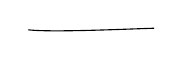
\begin{tikzpicture}\draw (0,0)..controls (.3,-.035) and (1.25,.01)..(1.6,.02);\end{tikzpicture}}

Je vois encore deux cas à regarder, savoir les sous-groupoïdes pleins de $\overline{\underline{\mathrm{VI}}}$ induits sur les \inserted{huit} sommets $(R_{i\omega},P^\omega)$, soit $\overline{\underline{\mathrm{VII}}}$, décrit par le graphe de $=$ nom et les flèches $d_i^{\prime\omega},d_i^\omega,a_i^\omega,b_i^\omega$ (24 flèches), et celui induit sur les \deleted{\unsure{cinq} points} \inserted{sommets} $Q_i,P^\omega$ --- à strictement parler, c'est le groupoïde déjà nommé $\overline{\underline{\mathrm{IV}}}$ ayant les $=$s \deleted{objets} sommets, mais
\figure{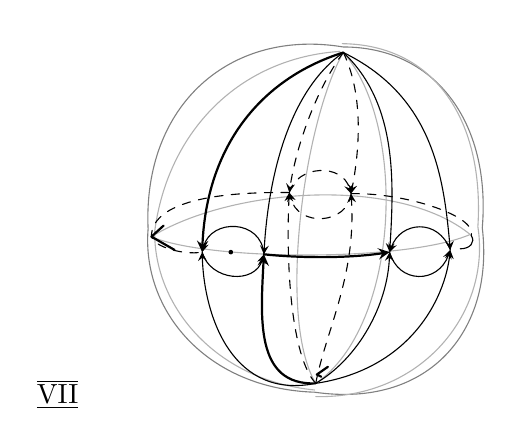
\begin{tikzpicture}[x=.014cm,y=-.014cm,line cap=round,line join=round,>=stealth]
\coordinate (N) at (192,18);\coordinate (S) at (167,318);
\coordinate (A) at (64,199);\coordinate (B) at (120,201);
\coordinate (C) at (143,145);\coordinate (D) at (199,146);
\coordinate (E) at (234,199);\coordinate (F) at (289,197);
\draw[gray,thin] (192,13)..controls (90,-4) and (10,65)..(15,178)..controls (9,253) and (69,323)..(166,326)..controls (270,341) and (329,270)..(318,177)..controls (326,81) and (275,13)..cycle;
\draw[gray!60,thin] (191,10)..controls (276,11) and (320,81)..(314,176)..controls (326,252) and (265,332)..(167,330);
\draw[gray!60,thin] (189,17)..controls (98,23) and (33,89)..(21,180)..controls (20,247) and (75,315)..(166,324);
\draw[gray!60,thin] (18,185)..controls (69,207) and (249,208)..(307,183);
\draw[gray!60,thin] (18,185)..controls (92,140) and (242,130)..(307,183);
\draw[gray!60,thin] (N)..controls (156,81) and (132,260)..(S);
\draw[gray!60,thin] (N)..controls (250,83) and (244,265)..(S);
\draw[thick,->] (N)..controls (116,42) and (68,104)..(A);
\draw[->] (N)..controls (142,53) and (124,132)..(B);
\draw[dashed,->] (N)..controls (167,52) and (149,104)..(C);
\draw[dashed,->] (N)..controls (209,53) and (208,100)..(D);
\draw[->] (N)..controls (241,64) and (238,135)..(E);
\draw[->] (N)..controls (274,58) and (283,132)..(F);
\draw[->] (S)..controls (93,333) and (66,260)..(A);
\draw[thick,->] (S)..controls (112,320) and (117,259)..(B);
\draw[dashed,->] (S)..controls (144,293) and (140,206)..(C);
\draw[thick] (178,303)--(168,310)--(172,312);
\draw[dashed,->] (S)..controls (176,271) and (204,220)..(D);
\draw[->] (S)..controls (206,295) and (232,247)..(E);
\draw[->] (S)..controls (253,305) and (284,241)..(F);
\draw[->] (B)..controls (118,169) and (72,168)..(A);
\draw[->] (A)..controls (71,225) and (112,229)..(B);
\draw[dashed,->] (C)..controls (150,120) and (191,118)..(D);
\draw[dashed,->] (D)..controls (196,174) and (151,177)..(C);
\draw[->] (F)..controls (278,168) and (244,171)..(E);
\draw[->] (E)..controls (242,228) and (278,228)..(F);
\draw[thick,->] (B)..controls (159,205) and (201,204)..(E);
\draw[dashed] (C)..controls (68,144) and (18,156)..(18,185)..controls (20,194) and (47,202)..(A);
\draw[thick] (29,175)--(18,185)--(39,197);
\draw[dashed] (D)..controls (250,145) and (314,167)..(308,184);
\draw (308,184)..controls (312,190) and (307,196)..(298,196);
\fill (90,199) circle (2.1);
\node at (-67,328) {$\overline{\underline{\mathrm{VII}}}$};
\end{tikzpicture}}
\margin{\uline{NB} les $b_i^\omega$ reliant directement les $Q_i$ sont ici inutiles}
\figure{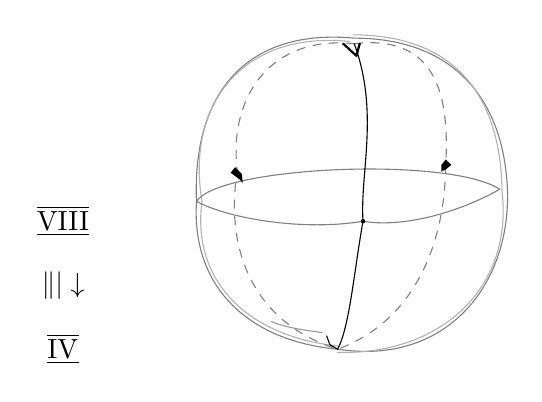
\begin{tikzpicture}[x=.014cm,y=-.014cm,line cap=round,line join=round,>=stealth]
\draw[gray,thin] (161,20)..controls (65,11) and (14,68)..(18,168)..controls (13,248) and (68,295)..(146,302)..controls (243,317) and (302,246)..(300,159)..controls (297,73) and (249,20)..cycle;
\draw[gray!60,thin] (160,17)..controls (252,17) and (294,72)..(295,159)..controls (305,243) and (244,307)..(146,305);
\draw[gray!60,thin] (157,23)..controls (61,13) and (8,79)..(23,168)..controls (13,242) and (67,291)..(146,299);
\draw[gray,thin] (18,168)..controls (39,136) and (247,127)..(293,157)..controls (254,179) and (204,192)..(169,186)..controls (116,195) and (48,184)..cycle;
\draw[gray,dashed] (161,25)..controls (82,17) and (47,77)..(55,140)..controls (43,215) and (72,279)..(146,302);
\draw[gray,dashed] (161,25)..controls (239,16) and (247,77)..(244,135)..controls (243,219) and (207,280)..(146,302);
\draw (161,25)..controls (184,87) and (166,143)..(169,186)..controls (161,230) and (157,281)..(146,302);
\draw[thick] (151,25)--(163,36)--(166,25);
\draw[gray!80] (86,277)..controls (100,283) and (119,285)..(132,287);
\draw (136,290)--(139,298)--(146,302);
\fill (53,137)--(49,142)--(57,148)--(60,151)--(59,143)--cycle;
\fill (244,130)--(240,135)--(240,141)--(244,139)--(249,135)--cycle;
\fill (169,186) circle (2.0);
\node at (-103,186) {$\overline{\underline{\mathrm{VIII}}}$};
\node at (-103,244) {$\unsure{\Vert|\downarrow}$};
\node at (-103,302) {$\overline{\underline{\mathrm{IV}}}$};
\end{tikzpicture}}
représenté par un graphe un peu plus grand --- dans $\boxed{\unsure{\mathrm{VIII}}}$ on distingue les \inserted{six} \(\underset{\rule{.5em}{.4pt}\quad\rule{.5em}{.4pt}\quad\rule{.5em}{.4pt}}{\text{\deleted{flèches}}}\) $d_i^\omega$ seulement, et on en donne \unsure{pas|par} en plus les $\widetilde a_i^\omega$, ce qui est inutile en \unsure{fait|effet} par (35). (Donc il n'est pas étonnant que dans (37), \unsure{\deleted{la}|la} donnée de $\widetilde\alpha$, qui
\margin{37}
